\documentclass[twoside]{book}

% Packages required by doxygen
\usepackage{fixltx2e}
\usepackage{calc}
\usepackage{doxygen}
\usepackage{graphicx}
\usepackage[utf8]{inputenc}
\usepackage{makeidx}
\usepackage{multicol}
\usepackage{multirow}
\PassOptionsToPackage{warn}{textcomp}
\usepackage{textcomp}
\usepackage[nointegrals]{wasysym}
\usepackage[table]{xcolor}

% Font selection
\usepackage[T1]{fontenc}
\usepackage{mathptmx}
\usepackage[scaled=.90]{helvet}
\usepackage{courier}
\usepackage{amssymb}
\usepackage{sectsty}
\renewcommand{\familydefault}{\sfdefault}
\allsectionsfont{%
  \fontseries{bc}\selectfont%
  \color{darkgray}%
}
\renewcommand{\DoxyLabelFont}{%
  \fontseries{bc}\selectfont%
  \color{darkgray}%
}
\newcommand{\+}{\discretionary{\mbox{\scriptsize$\hookleftarrow$}}{}{}}

% Page & text layout
\usepackage{geometry}
\geometry{%
  a4paper,%
  top=2.5cm,%
  bottom=2.5cm,%
  left=2.5cm,%
  right=2.5cm%
}
\tolerance=750
\hfuzz=15pt
\hbadness=750
\setlength{\emergencystretch}{15pt}
\setlength{\parindent}{0cm}
\setlength{\parskip}{0.2cm}
\makeatletter
\renewcommand{\paragraph}{%
  \@startsection{paragraph}{4}{0ex}{-1.0ex}{1.0ex}{%
    \normalfont\normalsize\bfseries\SS@parafont%
  }%
}
\renewcommand{\subparagraph}{%
  \@startsection{subparagraph}{5}{0ex}{-1.0ex}{1.0ex}{%
    \normalfont\normalsize\bfseries\SS@subparafont%
  }%
}
\makeatother

% Headers & footers
\usepackage{fancyhdr}
\pagestyle{fancyplain}
\fancyhead[LE]{\fancyplain{}{\bfseries\thepage}}
\fancyhead[CE]{\fancyplain{}{}}
\fancyhead[RE]{\fancyplain{}{\bfseries\leftmark}}
\fancyhead[LO]{\fancyplain{}{\bfseries\rightmark}}
\fancyhead[CO]{\fancyplain{}{}}
\fancyhead[RO]{\fancyplain{}{\bfseries\thepage}}
\fancyfoot[LE]{\fancyplain{}{}}
\fancyfoot[CE]{\fancyplain{}{}}
\fancyfoot[RE]{\fancyplain{}{\bfseries\scriptsize Generated on Mon Dec 8 2014 09\+:52\+:51 for Battle\+Ship (\+Project 2) by Doxygen }}
\fancyfoot[LO]{\fancyplain{}{\bfseries\scriptsize Generated on Mon Dec 8 2014 09\+:52\+:51 for Battle\+Ship (\+Project 2) by Doxygen }}
\fancyfoot[CO]{\fancyplain{}{}}
\fancyfoot[RO]{\fancyplain{}{}}
\renewcommand{\footrulewidth}{0.4pt}
\renewcommand{\chaptermark}[1]{%
  \markboth{#1}{}%
}
\renewcommand{\sectionmark}[1]{%
  \markright{\thesection\ #1}%
}

% Indices & bibliography
\usepackage{natbib}
\usepackage[titles]{tocloft}
\setcounter{tocdepth}{3}
\setcounter{secnumdepth}{5}
\makeindex

% Hyperlinks (required, but should be loaded last)
\usepackage{ifpdf}
\ifpdf
  \usepackage[pdftex,pagebackref=true]{hyperref}
\else
  \usepackage[ps2pdf,pagebackref=true]{hyperref}
\fi
\hypersetup{%
  colorlinks=true,%
  linkcolor=blue,%
  citecolor=blue,%
  unicode%
}

% Custom commands
\newcommand{\clearemptydoublepage}{%
  \newpage{\pagestyle{empty}\cleardoublepage}%
}


%===== C O N T E N T S =====

\begin{document}

% Titlepage & ToC
\hypersetup{pageanchor=false,
             bookmarks=true,
             bookmarksnumbered=true,
             pdfencoding=unicode
            }
\pagenumbering{roman}
\begin{titlepage}
\vspace*{7cm}
\begin{center}%
{\Large Battle\+Ship (Project 2) \\[1ex]\large 2.\+5.\+1 }\\
\vspace*{1cm}
{\large Generated by Doxygen 1.8.8}\\
\vspace*{0.5cm}
{\small Mon Dec 8 2014 09:52:51}\\
\end{center}
\end{titlepage}
\clearemptydoublepage
\tableofcontents
\clearemptydoublepage
\pagenumbering{arabic}
\hypersetup{pageanchor=true}

%--- Begin generated contents ---
\chapter{Hierarchical Index}
\section{Class Hierarchy}
This inheritance list is sorted roughly, but not completely, alphabetically\+:\begin{DoxyCompactList}
\item \contentsline{section}{Hit}{\pageref{class_hit}}{}
\begin{DoxyCompactList}
\item \contentsline{section}{W\+B\+Hit}{\pageref{class_w_b_hit}}{}
\end{DoxyCompactList}
\item \contentsline{section}{Legend}{\pageref{struct_legend}}{}
\end{DoxyCompactList}

\chapter{Class Index}
\section{Class List}
Here are the classes, structs, unions and interfaces with brief descriptions\+:\begin{DoxyCompactList}
\item\contentsline{section}{\hyperlink{struct_legend}{Legend} }{\pageref{struct_legend}}{}
\end{DoxyCompactList}

\chapter{Class Documentation}
\hypertarget{class_hit}{\section{Hit Class Reference}
\label{class_hit}\index{Hit@{Hit}}
}
Inheritance diagram for Hit\+:\begin{figure}[H]
\begin{center}
\leavevmode
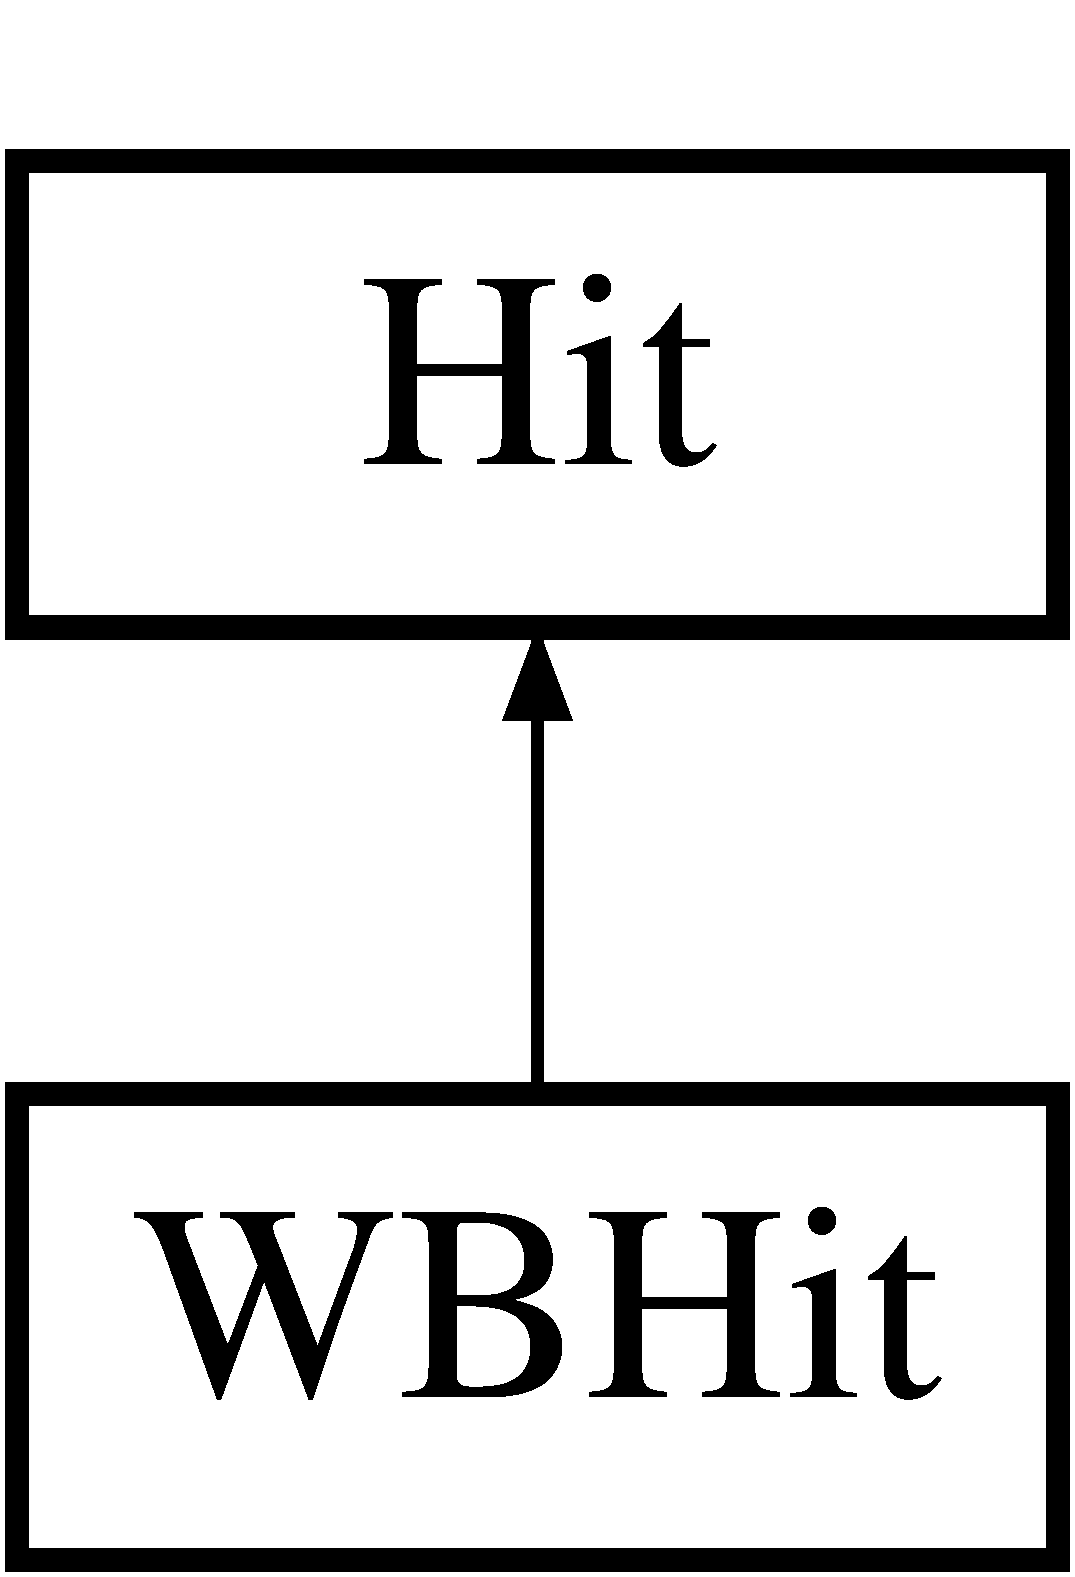
\includegraphics[height=2.000000cm]{class_hit}
\end{center}
\end{figure}
\subsection*{Public Member Functions}
\begin{DoxyCompactItemize}
\item 
\hypertarget{class_hit_a4564cb7f92efc815e5433a8593fd048f}{void {\bfseries set\+Err} ()}\label{class_hit_a4564cb7f92efc815e5433a8593fd048f}

\item 
\hypertarget{class_hit_a2bf9896f9e6c5749ea97027c004b33df}{string {\bfseries get\+Err} ()}\label{class_hit_a2bf9896f9e6c5749ea97027c004b33df}

\item 
\hypertarget{class_hit_af5ab95c622dbb5265d57228c0fc3e0ac}{virtual void {\bfseries get\+Hit} ()}\label{class_hit_af5ab95c622dbb5265d57228c0fc3e0ac}

\end{DoxyCompactItemize}


\subsection{Detailed Description}


Definition at line 20 of file Hit.\+h.



The documentation for this class was generated from the following files\+:\begin{DoxyCompactItemize}
\item 
Hit.\+h\item 
Hit.\+cpp\end{DoxyCompactItemize}

\hypertarget{struct_legend}{\section{Legend Struct Reference}
\label{struct_legend}\index{Legend@{Legend}}
}
\subsection*{Public Attributes}
\begin{DoxyCompactItemize}
\item 
string \hyperlink{struct_legend_aec74f6bcc74792152b73b2f20a00d6d3}{lgnd}
\item 
int \hyperlink{struct_legend_a9a061d9f5e944ca97358214e7c4e0d6b}{hit\+Mrk}
\item 
int \hyperlink{struct_legend_a637b6959e10df0779b48fdea71e7999d}{ship}
\end{DoxyCompactItemize}


\subsection{Detailed Description}


Definition at line 27 of file main.\+cpp.



\subsection{Member Data Documentation}
\hypertarget{struct_legend_a9a061d9f5e944ca97358214e7c4e0d6b}{\index{Legend@{Legend}!hit\+Mrk@{hit\+Mrk}}
\index{hit\+Mrk@{hit\+Mrk}!Legend@{Legend}}
\subsubsection[{hit\+Mrk}]{\setlength{\rightskip}{0pt plus 5cm}int Legend\+::hit\+Mrk}}\label{struct_legend_a9a061d9f5e944ca97358214e7c4e0d6b}


Definition at line 29 of file main.\+cpp.

\hypertarget{struct_legend_aec74f6bcc74792152b73b2f20a00d6d3}{\index{Legend@{Legend}!lgnd@{lgnd}}
\index{lgnd@{lgnd}!Legend@{Legend}}
\subsubsection[{lgnd}]{\setlength{\rightskip}{0pt plus 5cm}string Legend\+::lgnd}}\label{struct_legend_aec74f6bcc74792152b73b2f20a00d6d3}


Definition at line 28 of file main.\+cpp.

\hypertarget{struct_legend_a637b6959e10df0779b48fdea71e7999d}{\index{Legend@{Legend}!ship@{ship}}
\index{ship@{ship}!Legend@{Legend}}
\subsubsection[{ship}]{\setlength{\rightskip}{0pt plus 5cm}int Legend\+::ship}}\label{struct_legend_a637b6959e10df0779b48fdea71e7999d}


Definition at line 30 of file main.\+cpp.



The documentation for this struct was generated from the following file\+:\begin{DoxyCompactItemize}
\item 
\hyperlink{main_8cpp}{main.\+cpp}\end{DoxyCompactItemize}

\hypertarget{class_w_b_hit}{\section{W\+B\+Hit Class Reference}
\label{class_w_b_hit}\index{W\+B\+Hit@{W\+B\+Hit}}
}
Inheritance diagram for W\+B\+Hit\+:\begin{figure}[H]
\begin{center}
\leavevmode
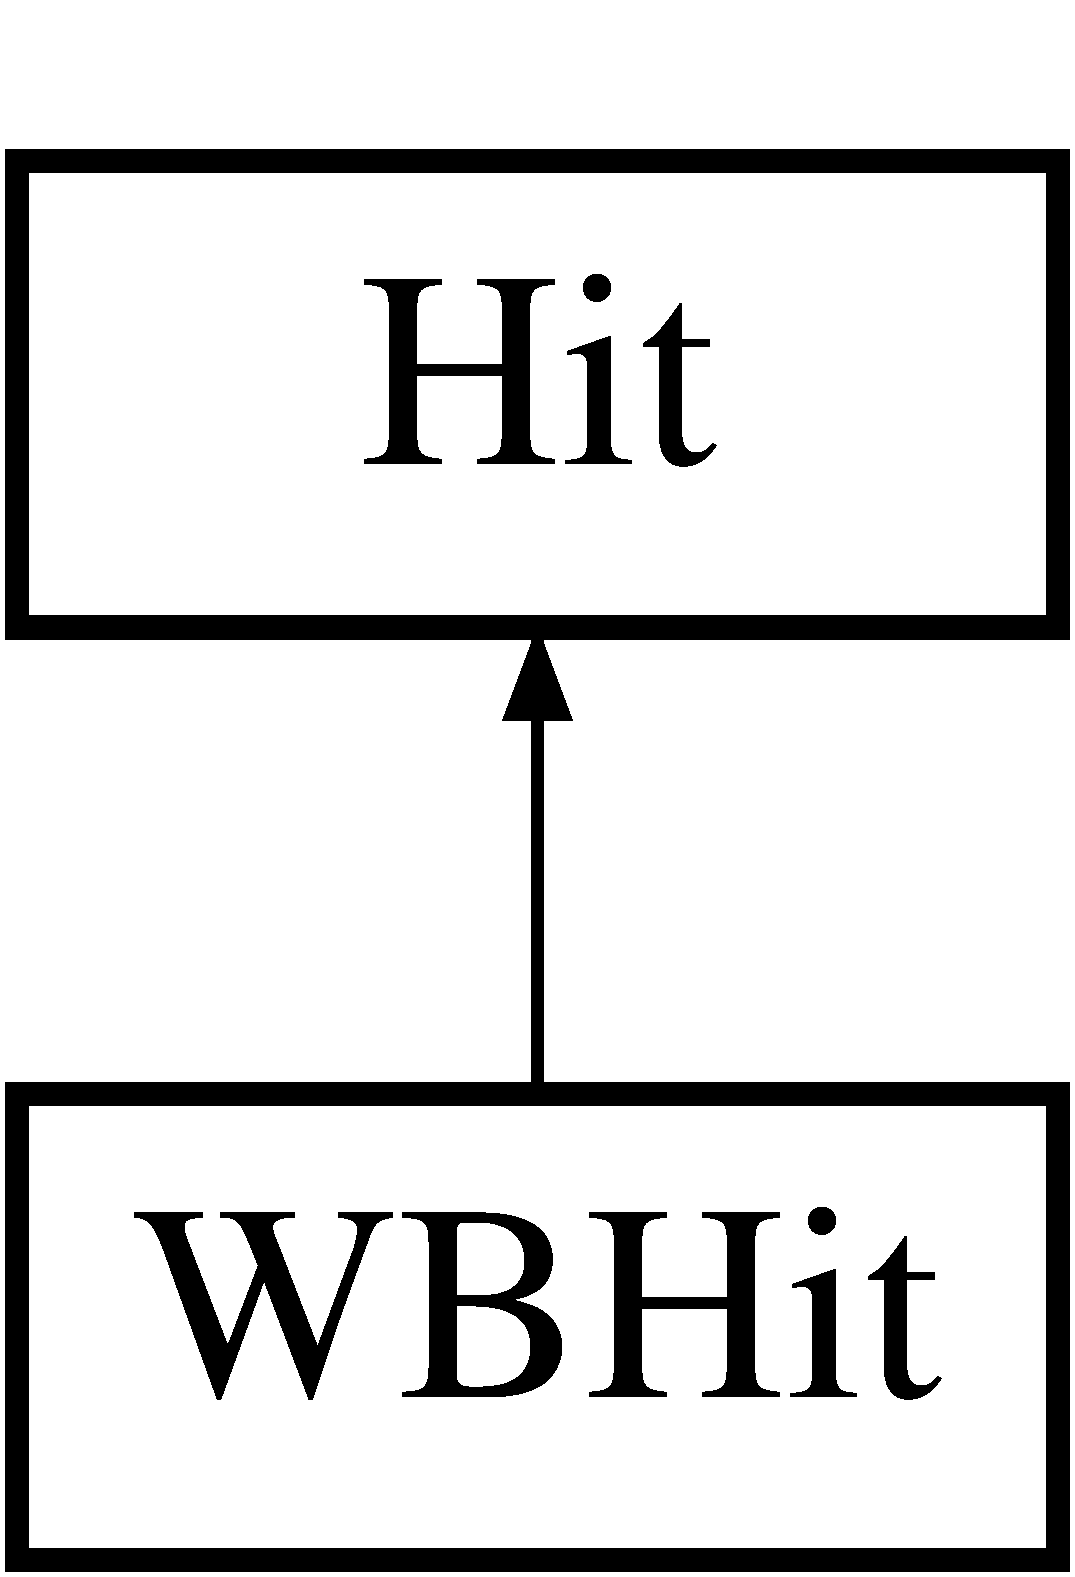
\includegraphics[height=2.000000cm]{class_w_b_hit}
\end{center}
\end{figure}
\subsection*{Public Member Functions}
\begin{DoxyCompactItemize}
\item 
\hypertarget{class_w_b_hit_a6b550026649e5d708282c364fa6e1acb}{bool {\bfseries is\+Read} ()}\label{class_w_b_hit_a6b550026649e5d708282c364fa6e1acb}

\item 
\hypertarget{class_w_b_hit_a33c27be52fde0db6ec41ef3f627f8976}{void {\bfseries get\+Hit} ()}\label{class_w_b_hit_a33c27be52fde0db6ec41ef3f627f8976}

\end{DoxyCompactItemize}


\subsection{Detailed Description}


Definition at line 19 of file W\+B\+Hit.\+h.



The documentation for this class was generated from the following files\+:\begin{DoxyCompactItemize}
\item 
W\+B\+Hit.\+h\item 
W\+B\+Hit.\+cpp\end{DoxyCompactItemize}

%--- End generated contents ---

% Index
\newpage
\phantomsection
\addcontentsline{toc}{chapter}{Index}
\printindex

\end{document}
